\chapter{Misura di resistenze con un multimetro digitale}\label{ch:mult}
    \lettrine[loversize=0.08, lines=2]{T}{ra le esperienze} svolte con il multimetro digitale riporto la misura delle resistenze di alcuni materiali, tra cui anelli metallici, il corpo umano e alcuni resistori.

    Ai resistori dedico una sezione più approfondita in quanto ho preso \num{50} misure su resistori distinti---ma teoricamente con resistenza uguale---per verificare la distribuzione delle misure di resistenza.

    \section{Il multimetro}
        Lo strumento utilizzato per l'interezza dell'esperienza è un multimetro digitale della serie \emph{DVM841} della \emph{Velleman\textsuperscript{\textregistered}} \cite{velleman-dvm841}. Il multimetro è in grado di misurare tensione e corrente continua e alternata, resistenza, frequenza e temperatura. Avendo una risoluzione di \num{2000} punti, il display del multimetro può visualizzare un massimo di \num{1999} unità.
    \section{Resistori}
        Il kit presenta $N = \num{50}$ resistori distinti---come quelli in \figref{fig:mul:resistore}---il cui codice colore restituisce un valore\footnote{Lo si può dedurre da qualunque legenda fedele allo standard IEC 60062.} teorico di $\SI{820}{\ohm} \pm \SI{5}{\%}$, ovvero \SI{820(40)}{\ohm}.
        \begin{figure}
            \centering
            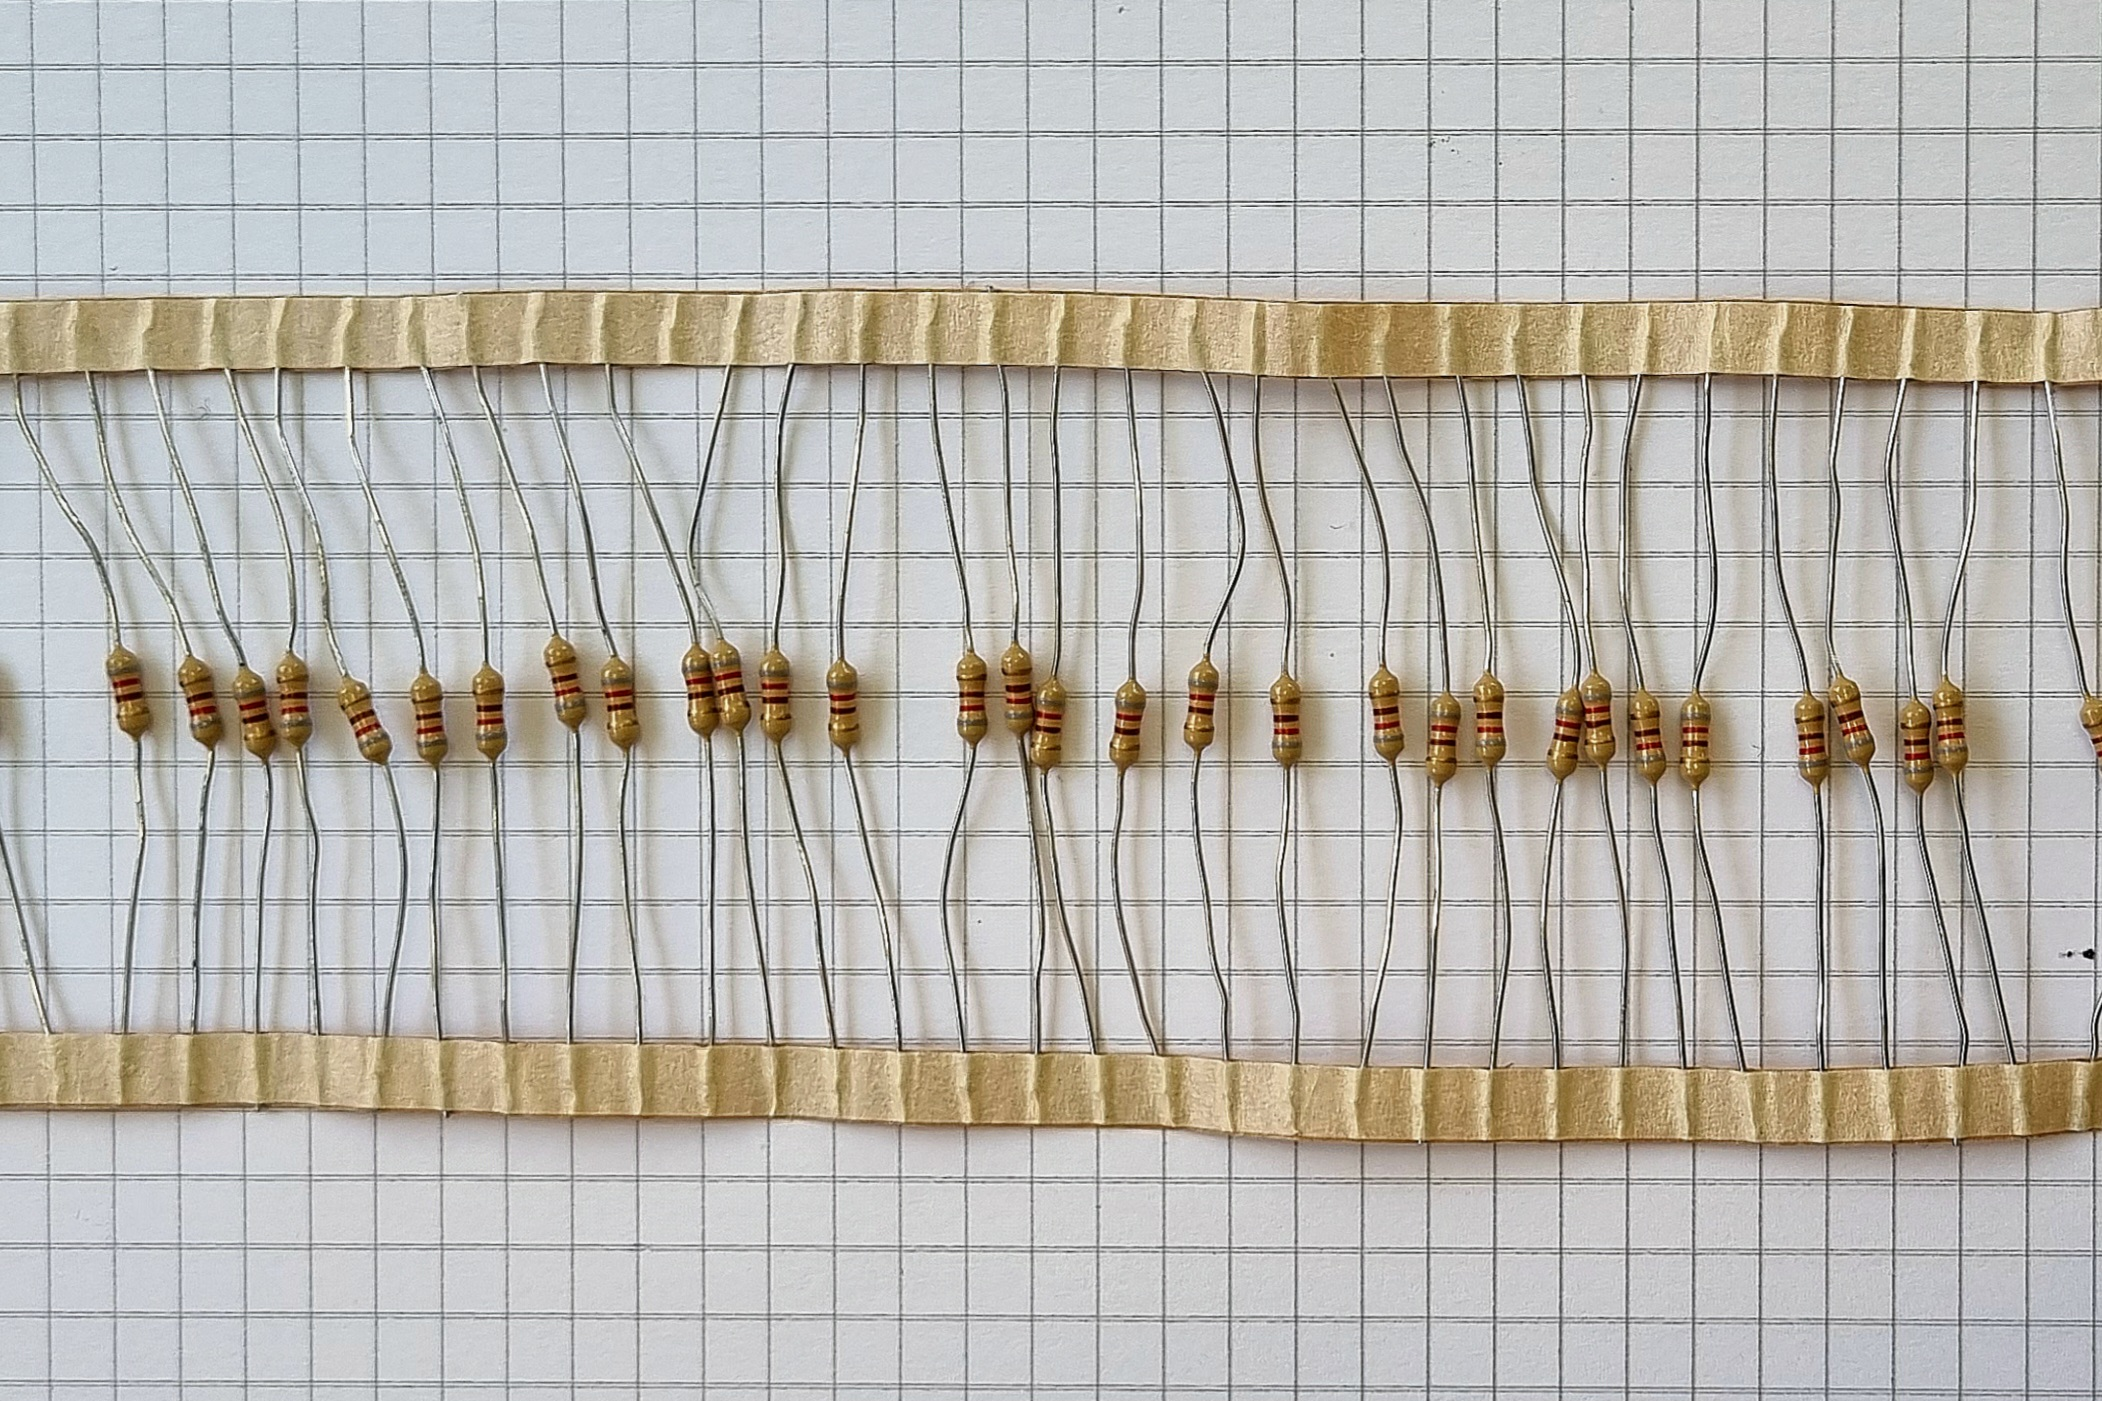
\includegraphics[width=0.4\textwidth]{images/multimetro/resistori.jpg}
            \hspace{0.05\textwidth}
            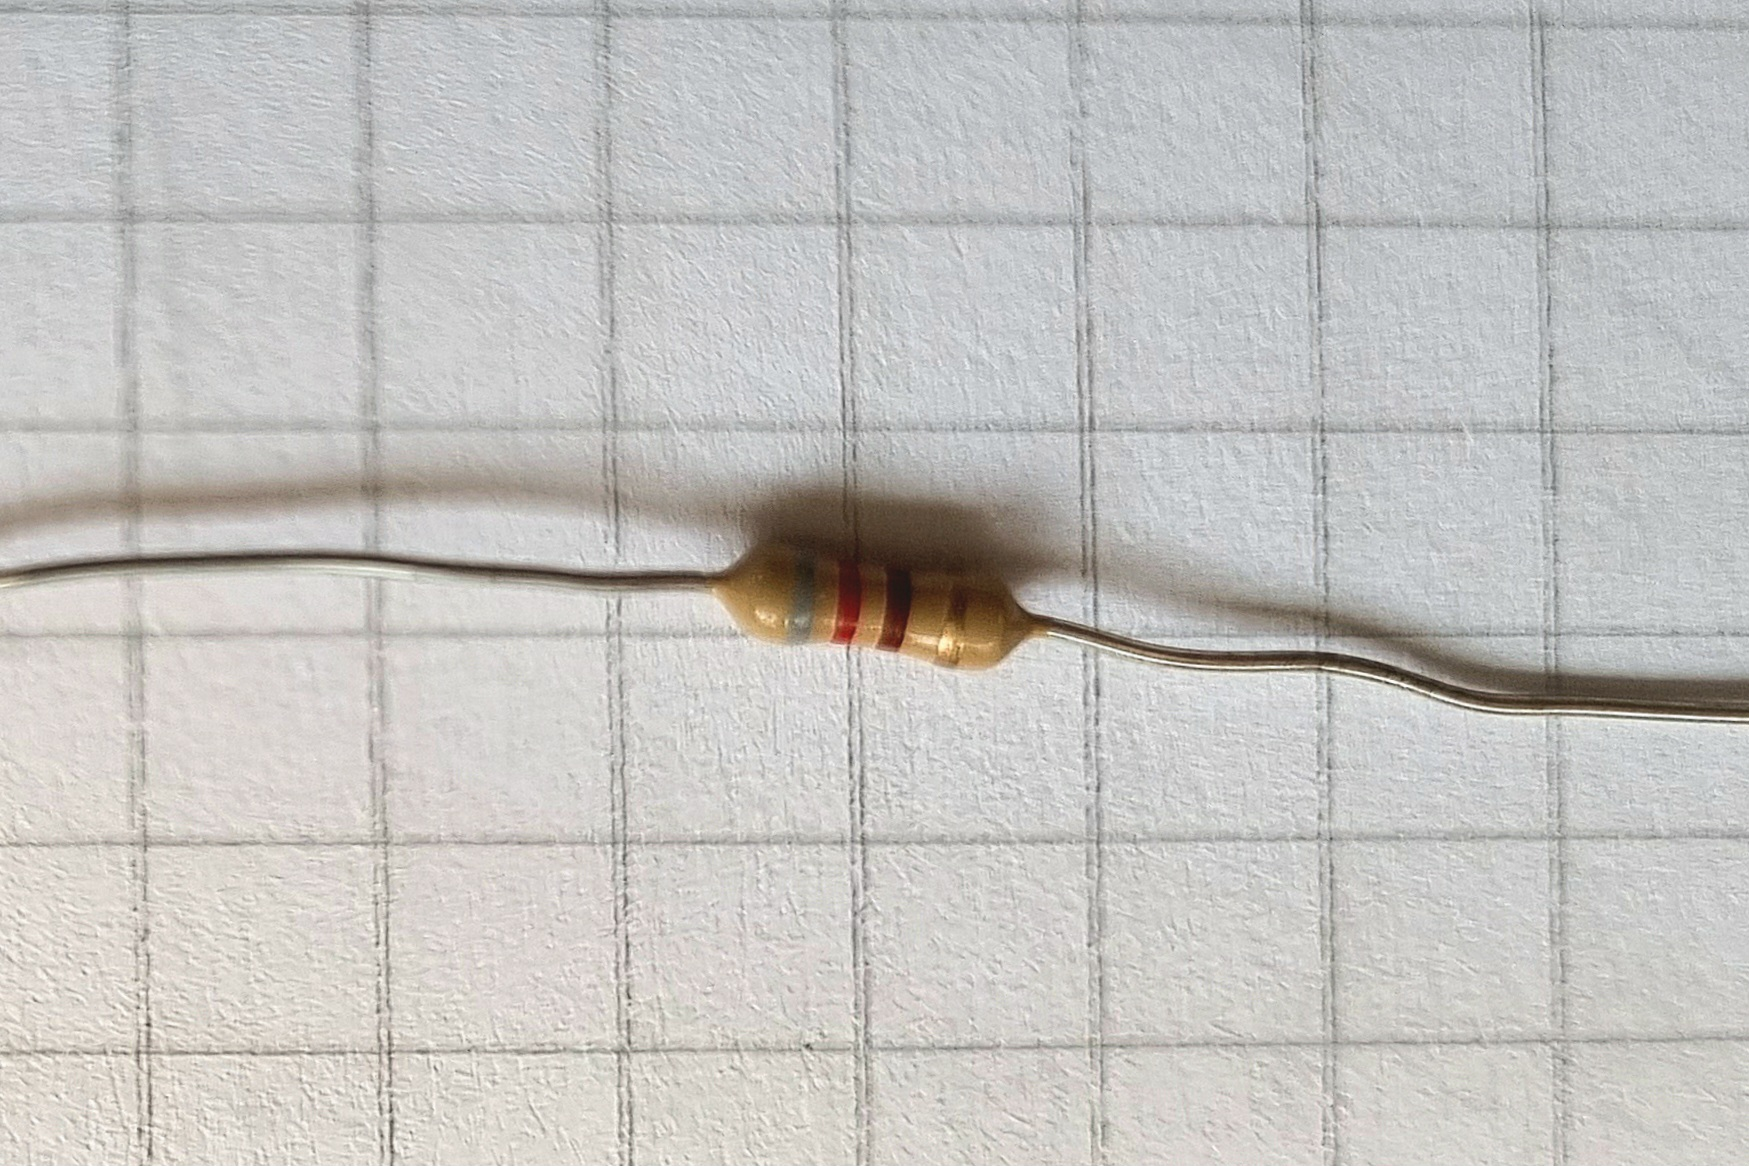
\includegraphics[width=0.4\textwidth]{images/multimetro/resistore.jpg}
            \caption{A sinistra alcuni dei \num{50} resistori da \SI{820}{\ohm}. A destra un dettaglio dove è visibile il codice colore.}
            \label{fig:mul:resistore}
        \end{figure}

        Ho effettuato le misure impostando il multimetro in modalità \emph{ohm}, alla portata di \SI{2}{\kilo\ohm}, poggiando i puntali sui terminali di ciascun resistore e aspettando di volta in volta che la lettura si stabilizzasse. I dati raccolti sono riportati in ordine crescente in \tabref{tab:mul:resistori}.
        \begin{table}
            \centering
            \begin{tabular}{cccccccccc}
    \hline
    \multicolumn{10}{c}{Resistenze (\unit{\ohm})}\\\hline\hline
    797 & 806 & 806 & 807 & 807 & 807 & 807 & 807 & 807 & 807 \\
    807 & 808 & 808 & 808 & 808 & 808 & 808 & 808 & 808 & 808 \\
    808 & 808 & 808 & 809 & 809 & 809 & 809 & 809 & 809 & 809 \\
    809 & 809 & 809 & 809 & 809 & 809 & 810 & 810 & 810 & 810 \\
    810 & 810 & 810 & 811 & 811 & 812 & 812 & 812 & 812 & 813 \\ \hline
\end{tabular}
            \caption{Misure di resistenza effettuate su \num{50} resistori distinti.}
            \label{tab:mul:resistori}
        \end{table}

        \subsection{Considerazioni preliminari}
            Notiamo subito che la resistenza media è $R_\text{m} = \SI{808.6}{\ohm}$ con una deviazione standard di $\sigma = \SI{2.3}{\ohm}$, l'errore sul valor medio è quindi $\sigma_R = \sigma / \sqrt{N-1} = \SI{0.33}{\ohm}$, che è confrontabile con la sensibilità dello strumento di \SI{1}{\ohm}.
            
            Questi valori rientrano completamete nell'intervallo fornito dal costruttore; tuttavia, il fatto che tutte le misure siano inferiori a \SI{820}{\ohm} suggerisce la presenza di un errore sistematico.\footnote{Se si trattasse di errori casuali dovuti a imprecisioni di fabbricazione, mi aspetterei letture sia al di sopra che al di sotto del valore di riferimento; è poco probabile che tutte le resistenze devino dal valore teorico allo stesso modo a meno che non si sia verificato un evento che ha alterato tutte le resistenze---un lotto prodotto con lo stesso materiale meno resistente, seppur entro il margine del \SI{5}{\%}, o deterioramento nel tempo.}

            Il dato di resistenza minima di \SI{797}{\ohm} può essere scartato secondo il cirerio di Chauvenet. Esso dista più di $4\sigma$ dal valor medio (ca. $\num{4.17}\sigma$) e il numero di dati atteso\footnote{Per il calcolo di questa probabilità ho fatto riferimento a [INSERIRE TAYLOR!!!]} su un campione di $N = 50$ elementi a una distanza maggiore o uguale a $4\sigma$ è pari a $\num{0.003} \ll 1/2$. Scartando questo dato la nuova media e la nuova deviazione standard sono:

        \subsection{Test del $\chi^2$}
            Supponiamo che le misure seguano la distribuzione normale centrata in $R_\text{m}$ e di ampiezza $\sigma$:
            \begin{equation*}
                N\pqty{x; R_\text{m}, \sigma}
                = \frac{1}{\sqrt{2\pi\sigma^2}} \exp[ -\frac{1}{2}\pqty{\frac{x - R_\text{m}}{\sigma}}^2]
                \myperiod
            \end{equation*}
            
            Costruiamo quindi un istogramma dei dati. Visto l'intervallo contenuto in cui le misure variano, ho scelto di raccogliere i dati in bin di ampiezza \SI{1}{\ohm}, uno per ciascun valore misurato; ciascun bin si estende da mezza unità \emph{prima} del valore di interesse a mezza unità \emph{dopo}. In \tabref{tab:mul:bin-istogramma} sono riportati i bin e le frequenze osservate $O_k$.
            \begin{table}
                \centering
                \begin{tabular}{ccccc|rc}\hline
    \multicolumn{5}{c}{Intervalli}                  & $O_k$    & $E_k$       \\
    \hline\hline
                  &     & $R$ & $<$ & $\num{806.5}$ & \num{2}  & \num{4.133} \\
    $\num{806.5}$ & $<$ & $R$ & $<$ & $\num{807.5}$ & \num{8}  & \num{5.735} \\
    $\num{807.5}$ & $<$ & $R$ & $<$ & $\num{808.5}$ & \num{12} & \num{6.925} \\
    $\num{808.5}$ & $<$ & $R$ & $<$ & $\num{809.5}$ & \num{13} & \num{7.278} \\
    $\num{809.5}$ & $<$ & $R$ & $<$ & $\num{810.5}$ & \num{6}  & \num{6.655} \\
    $\num{810.5}$ & $<$ & $R$ & $<$ & $\num{811.5}$ & \num{2}  & \num{5.297} \\
    $\num{811.5}$ & $<$ & $R$ & $<$ & $\num{812.5}$ & \num{4}  & \num{3.668} \\
    $\num{812.5}$ & $<$ & $R$ &     &               & \num{1}  & \num{2.211} \\
    \hline
\end{tabular}
                \caption{Suddivisione dei dati per il test del $\chi^2$. Ometto le unità di misura per chiarezza espositiva e semplicità dei calcoli.}
                \label{tab:mul:bin-istogramma}
            \end{table}

            Da qui eseguo il test nell'usuale modo: converto gli esetremi dell'intervallo in variabili normali standardizzate sottraendo la media e dividendo per la deviazione standard, attraverso un foglio di calcolo trovo il valore dell'integrale della gaussiana per ciascun intervallo, moltiplico tale valore per la dimensione del campione $N = 49$ per trovare i valori attesi $E_k$.